\documentclass{article}
\usepackage[utf8]{inputenc}
\usepackage{hyperref}
\usepackage{amsmath}
\usepackage{amssymb}
\usepackage{geometry}
\usepackage{graphicx}
\usepackage{float}
\usepackage{fancyhdr}
\usepackage{listings}
\usepackage{float}

\pagestyle{fancy}
\fancyhf{}
\fancyhead[L]{Conception de Base de Données - TP2}
\fancyhead[R]{SANNA Thomas, L3STI}
\fancyfoot[C]{Page n°\thepage}
\fancyfoot[R]{Università di Corsica}

\title{Conception de Base de Données: \\ TP2 - Exercices}
\author{SANNA Thomas}
\date{\today}

\begin{document}

\begin{figure}
  \centering
  
\includegraphics[width=0.5\textwidth]{img/logoUniv.jpg}
  \label{fig:mysql-logo}
\end{figure}

\maketitle

\break\tableofcontents

\break\section{Exercice 1 (A)}

\subsection{Modèle Conceptuel de Données (MCD)}

\begin{figure}[H]
  \centering
  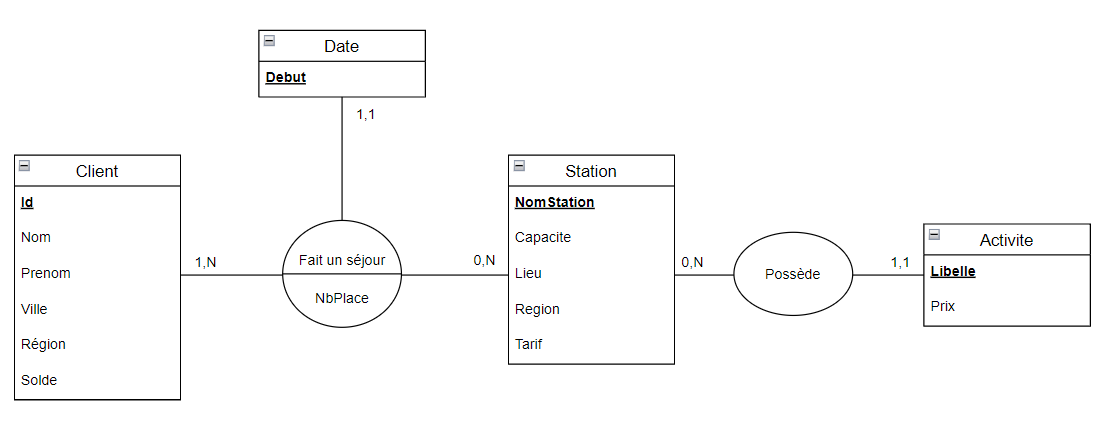
\includegraphics[width=1\textwidth]{imgMcd/mcd.png}
  \caption{Modèle Conceptuel de Données, en utilisant Draw.io.}
  \label{fig:MCD}
\end{figure}

\subsection{Couverture Minimale}

\begin{figure}[H]
  \centering
  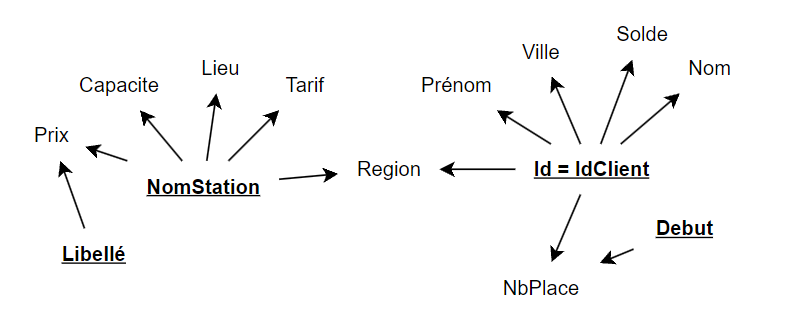
\includegraphics[width=0.8\textwidth]{imgMcd/couvMin.png}
  \caption{Couverture Minimale, en utilisant Draw.io.}
  \label{fig:CM}
\end{figure}

\break\section{Exercice 2 (B)}

$ Station (Nomstation, Capacite, Lieu, Region, Tarif) $

$ Activite (\#NomStation, Libelle, Prix) $

$ Client (Id, Nom, Prenom, Ville, Region, Solde) $

$ Sejour (\#IdClient, \#NomStation, Debut, Nbplace) $

\subsection{Toutes les stations aux Antilles}

$ R1 = \sigma_{region = 'Antilles'}(Station)$

\begin{figure}[H]
  \centering
  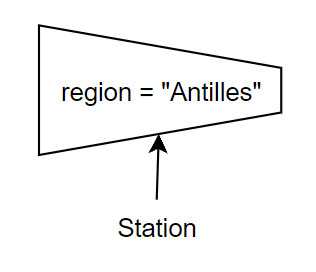
\includegraphics[width=0.3\textwidth]{imgAlgGraph/1.png}
  \label{fig:1}
\end{figure}

\subsection{Donner le nom des stations et leur région}

$ R1 = \pi_{nomStation, region}(Station)$

\begin{figure}[H]
  \centering
  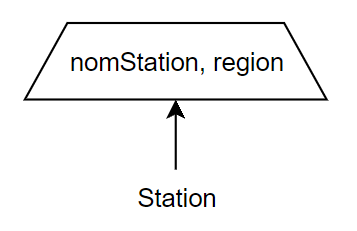
\includegraphics[width=0.3\textwidth]{imgAlgGraph/2.png}
  \label{fig:2}
\end{figure}

\subsection{Donner toutes les régions où il y a des stations}

$ R1 = \pi_{region}(Station)$

\begin{figure}[H]
  \centering
  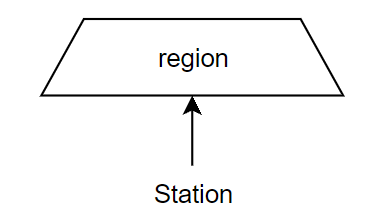
\includegraphics[width=0.3\textwidth]{imgAlgGraph/3.png}
  \label{fig:3}
\end{figure}

\subsection{Donner toutes les stations qui sont aux Antilles et dont la capacité est supérieure à 200}

$ R1 = \sigma_{region = 'Antilles' \wedge capacite > 200}(Station)$

\begin{figure}[H]
  \centering
  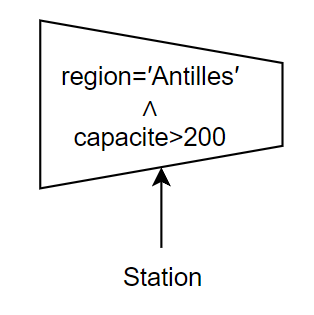
\includegraphics[width=0.3\textwidth]{imgAlgGraph/4.png}
  \label{fig:4}
\end{figure}

\subsection{Donner toutes les stations qui sont aux Antilles ou dont la capacité est supérieure à 200}

$ R1 = \sigma_{region = 'Antilles' \vee capacite > 200}(Station)$

\begin{figure}[H]
  \centering
  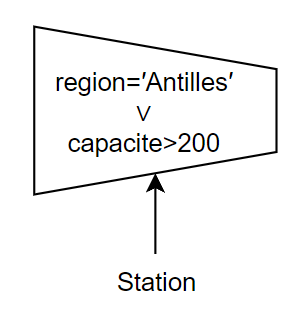
\includegraphics[width=0.3\textwidth]{imgAlgGraph/5.png}
  \label{fig:5}
\end{figure}

\subsection{Donner toutes les stations dont la capacité est supérieure à 200 mais qui ne sont pas aux Antilles}

$ R1 = \sigma_{capacite > 200 \wedge region \neq 'Antilles'}(Station)$

\begin{figure}[H]
  \centering
  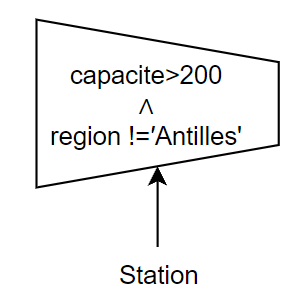
\includegraphics[width=0.3\textwidth]{imgAlgGraph/6.png}
  \label{fig:6}
\end{figure}

\subsection{Donner le nom des stations aux Antilles}

$ R1 = \sigma_{region = 'Antilles'}(Station)$

$ R2 = \pi_{nomStation}(R1)$

\begin{figure}[H]
  \centering
  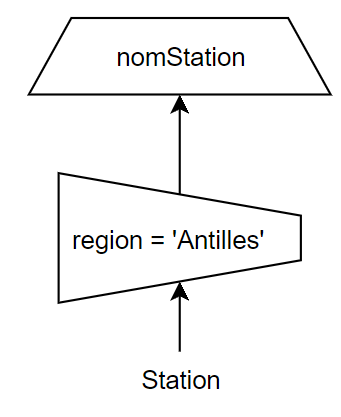
\includegraphics[width=0.3\textwidth]{imgAlgGraph/7.png}
  \label{fig:7}
\end{figure}

\subsection{Donner le nom des stations où on pratique la plongée}

$ R1 = \sigma_{libelle = \text{'Plongée'}}(Activite)$

$ R2 = \pi_{nomStation}(R1)$

\begin{figure}[H]
  \centering
  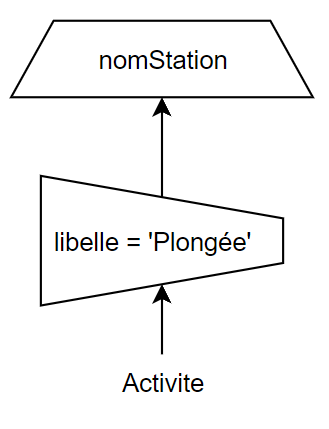
\includegraphics[width=0.3\textwidth]{imgAlgGraph/8.png}
  \label{fig:8}
\end{figure}

\subsection{Donner le nom et le prénom des clients européens}

$ R1 = \sigma_{region = \text{'Europe'}}(Client)$

$ R2 = \pi_{id, nom, prenom}(R1)$

\begin{figure}[H]
  \centering
  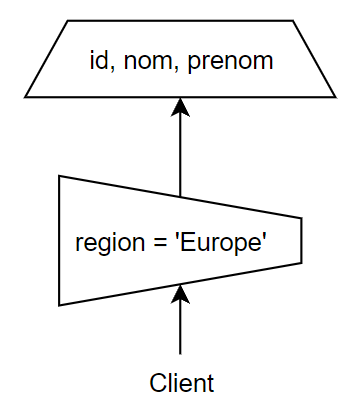
\includegraphics[width=0.3\textwidth]{imgAlgGraph/9.png}
  \label{fig:9}
\end{figure}

\subsection{Donner le nom des clients ayant fait des séjours en 2019}

$ R1 = \sigma_{debut = \text{'2019'}}(Sejour)$

$ R2 = \pi_{idClient}(R1)$

$ R3 = (R2)idClient \Join id(Client)$

$ R4 = \pi_{idClient, nom}(R3)$

\begin{figure}[H]
  \centering
  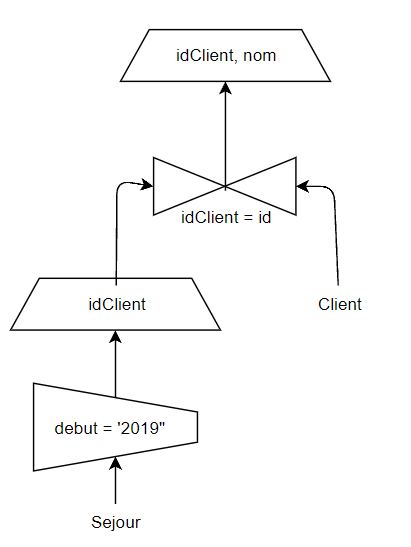
\includegraphics[width=0.4\textwidth]{imgAlgGraph/10.png}
  \label{fig:10}
\end{figure}

\subsection{Donner le nom et la région des stations où on pratique la voile}

$ R1 = \sigma_{libelle = \text{'Voile'}}(Activite)$

$ R2 = \pi_{nomStation}(R1)$

$ R3 = (R2)nomStation \Join nomStation(Station)$

$ R4 = \pi_{nomStation, region}(R3)$

\begin{figure}[H]
  \centering
  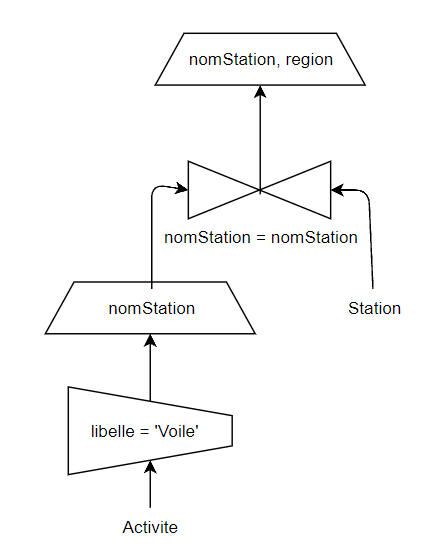
\includegraphics[width=0.4\textwidth]{imgAlgGraph/11.png}
  \label{fig:11}
\end{figure}

\subsection{Donner le nom des clients qui sont allés à Santalba}

$ R1 = \sigma_{nomStation = \text{'Santalba'}}(Sejour)$

$ R2 = \pi_{idClient}(R1)$

$ R3 = (R2)idClient \Join id(Client)$

$ R4 = \pi_{idClient, nom}(R3)$

\begin{figure}[H]
  \centering
  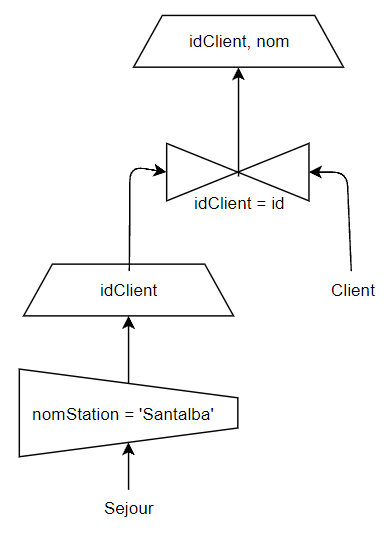
\includegraphics[width=0.4\textwidth]{imgAlgGraph/12.png}
  \label{fig:12}
\end{figure}

\subsection{Donner les régions visitées par le client 30}

$ R1 = \sigma_{idClient = 30}(Sejour)$

$ R2 = \pi_{nomStation}(R1)$

$ R3 = (R2)nomStation \Join nomStation(Station)$

$ R4 = \pi_{region}(R3)$

\begin{figure}[H]
  \centering
  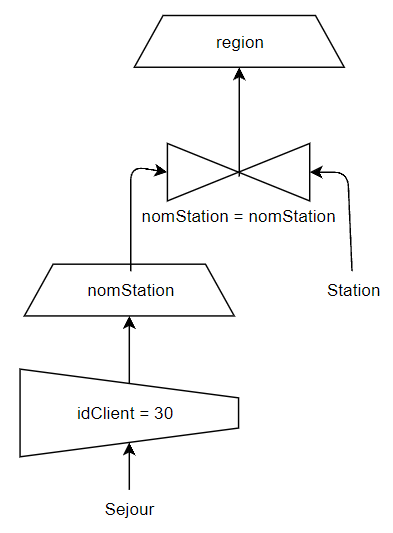
\includegraphics[width=0.4\textwidth]{imgAlgGraph/13.png}
  \label{fig:13}
\end{figure}

\subsection{Donner le nom des clients qui ont eu l’occasion de faire de la Plongée}

$ R1 = \sigma_{libelle = \text{'Plongée'}}(Activite)$

$ R2 = \pi_{nomStation}(R1)$

$ R3 = (R2)nomStation \Join nomStation(Sejour)$

$ R4 = \pi_{idClient}(R3)$

$ R5 = (R4)idClient \Join id(Client)$

$ R6 = \pi_{idClient, nom}(R5)$

\begin{figure}[H]
  \centering
  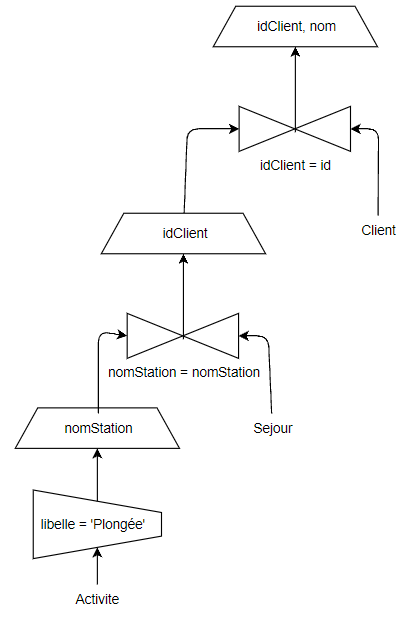
\includegraphics[width=0.5\textwidth]{imgAlgGraph/14.png}
  \label{fig:14}
\end{figure}

\subsection{Donner les régions où il y a des clients mais pas de stations}

$ R1 = \pi_{region}(Client)$

$ R2 = \pi_{region}(Station)$

$ R3 = R1 - R2$

\begin{figure}[H]
  \centering
  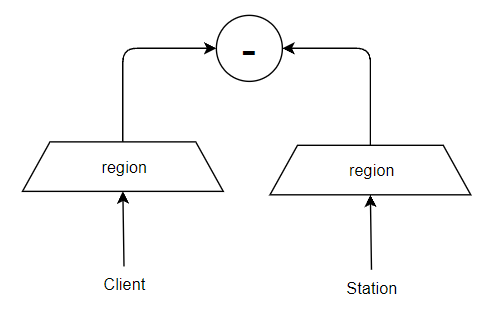
\includegraphics[width=0.3\textwidth]{imgAlgGraph/15.png}
  \label{fig:15}
\end{figure}

\subsection{Donner les noms des stations qui n’ont pas reçu de client américain}

$ R1 = \sigma_{region = \text{'Amerique'}}(Client)$

$ R2 = \pi_{id}(R1)$

$ R3 = (R2)id \Join idClient(Sejour)$

$ R4 = \pi_{nomStation}(R3)$

$ R5 = \pi_{nomStation}(Station) - R4$

\begin{figure}[H]
  \centering
  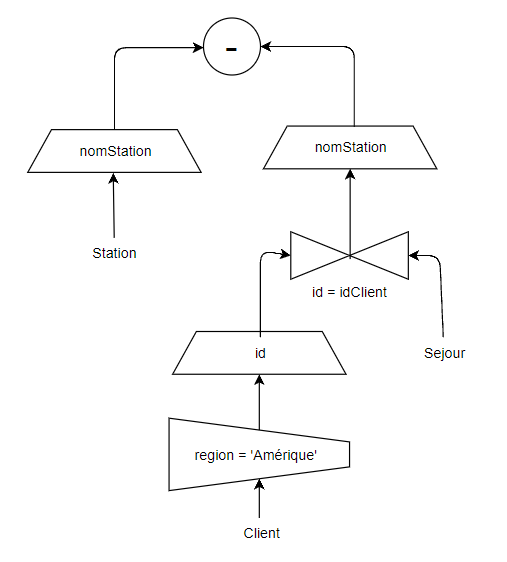
\includegraphics[width=0.4\textwidth]{imgAlgGraph/16.png}
  \label{fig:16}
\end{figure}

\subsection{Quelles sont les stations dont toutes les activités ont un prix supérieur à 100 (équivalent à quelles sont les stations pour lesquelles il n’existe pas de prix inférieur à 100)}

$ R1 = \sigma_{prix < 100}(Activite)$

$ R2 = \pi_{nomStation}(R1)$

$ R3 = \pi_{nomStation}(Station) - R2$

\begin{figure}[H]
  \centering
  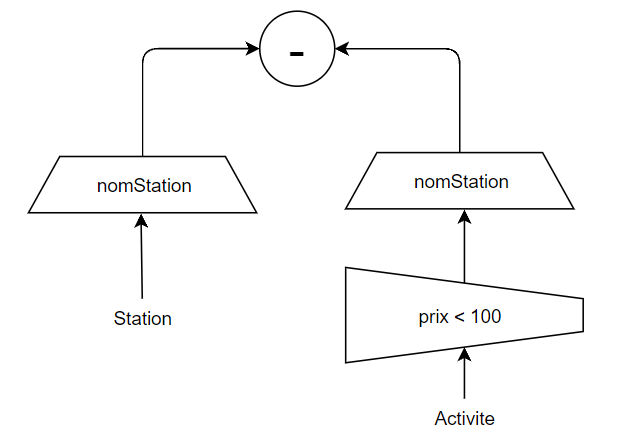
\includegraphics[width=0.3\textwidth]{imgAlgGraph/17.png}
  \label{fig:17}
\end{figure}

\section{Exercice 3 (C)}

\subsection*{Création de la base de données mysql:}

\begin{lstlisting}[language=SQL]

CREATE TABLE IF NOT EXISTS `station` (
  `nomStation` VARCHAR(50) NOT NULL,
  `capacite` INT(11) NOT NULL,
  `lieu` VARCHAR(50) NOT NULL,
  `region` VARCHAR(50) NOT NULL,
  `tarif` INT(11) NOT NULL,
  PRIMARY KEY (`nomStation`)
) ENGINE=InnoDB DEFAULT CHARSET=utf8;

CREATE TABLE IF NOT EXISTS `activite` (
  `nomStation` VARCHAR(50) NOT NULL,
  `libelle` VARCHAR(50) NOT NULL,
  `prix` INT(11) NOT NULL,
  PRIMARY KEY (`nomStation`, `libelle`),
  CONSTRAINT `activite_ibfk_1` FOREIGN KEY (`nomStation`) REFERENCES `station` (`nomStation`)
) ENGINE=InnoDB DEFAULT CHARSET=utf8;

CREATE TABLE IF NOT EXISTS `client` (
  `id` INT(11) NOT NULL AUTO_INCREMENT,
  `nom` VARCHAR(50) NOT NULL,
  `prenom` VARCHAR(50) NOT NULL,
  `ville` VARCHAR(50) NOT NULL,
  `region` VARCHAR(50) NOT NULL,
  `solde` INT(11) NOT NULL,
  PRIMARY KEY (`id`)
) ENGINE=InnoDB DEFAULT CHARSET=utf8;

CREATE TABLE IF NOT EXISTS `sejour` (
  `idClient` INT(11) NOT NULL,
  `nomStation` VARCHAR(50) NOT NULL,
  `debut` DATE NOT NULL,
  `nbplace` INT(11) NOT NULL,
  PRIMARY KEY (`idClient`, `nomStation`),
  CONSTRAINT `sejour_ibfk_1` FOREIGN KEY (`idClient`) REFERENCES `client` (`id`),
  CONSTRAINT `sejour_ibfk_2` FOREIGN KEY (`nomStation`) REFERENCES `station` (`nomStation`)
) ENGINE=InnoDB DEFAULT CHARSET=utf8;

\end{lstlisting}

\subsection{Toutes les stations aux Antilles}

\begin{lstlisting}[language=SQL]

SELECT * 
FROM station 
WHERE region = 'Antilles';

\end{lstlisting}

\subsection{Donner le nom des stations et leur région}

\begin{lstlisting}[language=SQL]

SELECT nomStation, region 
FROM station;

\end{lstlisting}

\subsection{Donner toutes les régions où il y a des stations}

\begin{lstlisting}[language=SQL]

SELECT DISTINCT region 
FROM station;

\end{lstlisting}

\subsection{Donner toutes les stations qui sont aux Antilles et dont la capacité est supérieure à 200}

\begin{lstlisting}[language=SQL]

SELECT * 
FROM station 
WHERE region = 'Antilles' AND capacite > 200;

\end{lstlisting}

\subsection{Donner toutes les stations qui sont aux Antilles ou dont la capacité est supérieure à 200}

\begin{lstlisting}[language=SQL]

SELECT * 
FROM station 
WHERE region = 'Antilles' OR capacite > 200;

\end{lstlisting}

\subsection{Donner toutes les stations dont la capacité est supérieure à 200 mais qui ne sont pas aux Antilles}

\begin{lstlisting}[language=SQL]

SELECT * 
FROM station 
WHERE capacite > 200 AND region != 'Antilles';

\end{lstlisting}

\subsection{Donner le nom des stations aux Antilles}

\begin{lstlisting}[language=SQL]

SELECT nomStation 
FROM station WHERE region = 'Antilles';

\end{lstlisting}

\subsection{Donner le nom des stations où on pratique la plongée}

\begin{lstlisting}[language=SQL]

SELECT nomStation 
FROM activite 
WHERE libelle = 'Plongee';

\end{lstlisting}

\subsection{Donner le nom et le prénom des clients européens}

\begin{lstlisting}[language=SQL]

SELECT id, nom, prenom 
FROM client 
WHERE region = 'Europe';

\end{lstlisting}

\subsection{Donner le nom des clients ayant fait des séjours en 2019}

\begin{lstlisting}[language=SQL]

SELECT client.id, client.nom 
FROM sejour 
JOIN client ON sejour.idClient = client.id 
WHERE YEAR(sejour.debut) = 2019;

\end{lstlisting}

\subsection{Donner le nom et la région des stations où on pratique la voile}

\begin{lstlisting}[language=SQL]

SELECT station.nomStation, station.region 
FROM activite 
JOIN station ON activite.nomStation = station.nomStation 
WHERE activite.libelle = 'Voile';

\end{lstlisting}

\subsection{Donner le nom des clients qui sont allés à Santalba}

\begin{lstlisting}[language=SQL]

SELECT client.id, client.nom
FROM sejour
JOIN client ON sejour.idClient = client.id
WHERE sejour.nomStation = 'Santalba';

\end{lstlisting}

\subsection{Donner les régions visitées par le client 30}

\begin{lstlisting}[language=SQL]

SELECT DISTINCT station.region
FROM sejour
JOIN station ON sejour.nomStation = station.nomStation
WHERE sejour.idClient = 30;

\end{lstlisting}

\subsection{Donner le nom des clients qui ont eu l’occasion de faire de la Plongée}

\begin{lstlisting}[language=SQL]

SELECT client.id, client.nom
FROM activite
JOIN sejour ON activite.nomStation = sejour.nomStation
JOIN client ON sejour.idClient = client.id
WHERE activite.libelle = 'Plongee';

\end{lstlisting}

\subsection{Donner les régions où il y a des clients mais pas de stations}

\begin{lstlisting}[language=SQL]

SELECT DISTINCT client.region
FROM client
LEFT JOIN sejour ON client.id = sejour.idClient
WHERE sejour.nomStation IS NULL;

\end{lstlisting}

\subsection{Donner les noms des stations qui n’ont pas reçu de client américain}

\begin{lstlisting}[language=SQL]

SELECT station.nomStation
FROM station
LEFT JOIN sejour ON station.nomStation = sejour.nomStation
LEFT JOIN client ON sejour.idClient = client.id
WHERE client.region != 'Amerique';

\end{lstlisting}

\subsection{Quelles sont les stations dont toutes les activités ont un prix supérieur à 100}

\begin{lstlisting}[language=SQL]

SELECT station.nomStation
FROM station
LEFT JOIN activite ON station.nomStation = activite.nomStation
WHERE activite.prix < 100;

\end{lstlisting}


\end{document}